% Working Chapter 2, 2026-10-24. Source/evidence records: planning/verification-background.md.
% HyperKG evidence uses the author's confirmed publication-equivalent arXiv PDF.
\chapter{Background and Related Work}
\label{ch:background}

The methods in this thesis use structure to determine which information a language model receives and how that information enters prediction. Their structures have different origins. A knowledge graph records external entities and relations; a classification index connects keywords with labels; an evidence graph links facts and passages; and a query graph expresses the relationships requested by a question. This chapter establishes the concepts needed to compare these representations and reviews work on table understanding, retrieval-augmented generation, graph retrieval, and multimodal context processing. Section~\ref{sec:background:hyperkg} presents the author's published study of information preservation in hyper-relational knowledge graphs.

\section{Knowledge Graphs and Language Models}
\label{sec:background:knowledge-models}

A knowledge graph represents entities and their relationships explicitly. In a conventional relational representation, a fact is a triple $(s,r,o)$, where $s$ is a subject entity, $r$ a relation, and $o$ an object entity. A set of these facts forms a directed graph whose edge labels identify relations. Wikidata provides a collaborative knowledge resource in which structured statements and their qualifiers can describe entities beyond the content of a single document~\cite{bg-wikidata}. A model accessing this graph can retrieve relations associated with a mentioned entity, including information absent from its immediate input.

The graph representation separates an entity's identity from the strings used to mention it. A table cell or query contains a mention, while an entity node refers to an indexed object. Entity linking establishes a correspondence between the two. A short name may match several entities, so a retrieval score and a contextual disambiguation rule can influence which facts become available. The distinction remains relevant when a graph is extracted from text: repeated strings, aliases, and synonyms affect whether different passages share a node. These indexing choices determine possible paths before a query-specific selection algorithm begins.

Graph topology records the connections available to a computation. A neighborhood identifies adjacent entities and relations; a path composes a sequence of such connections; and a subgraph retains a selected set of nodes and edges. These objects support different operations. Neighborhood aggregation can enrich an entity representation, a path can provide evidence connecting two mentioned entities, and a subgraph can organize several facts relevant to a question. Their usefulness depends on the interpretation of the edges. A factual relation, a lexical-similarity edge, and a keyword--label association impose different meanings on a traversed connection.

Language models provide a complementary representation. The Transformer uses attention to compute token representations from their context~\cite{bg-transformer}. BERT pre-trains bidirectional contextual representations and can be fine-tuned with a task-specific output layer~\cite{bg-bert}. In column annotation, contextual token vectors can represent a column and feed a classifier. Generative language models instead produce an answer sequence conditioned on the query and supplied context. This thesis uses the term language model for both roles and specifies the relevant prediction interface in each research chapter.

Knowledge stored in learned parameters and evidence supplied at prediction time enter these interfaces differently. Fine-tuning modifies model parameters using labeled examples. Retrieval selects material from an external index and places it in the model's input. A model can combine both, as in KGLink's learned annotation model with graph-derived features. The later RAG systems emphasize the selection of external evidence for a generator. Comparing these methods therefore requires identifying the source of evidence, the operation that selects it, and the model component that uses the selected representation.

\section{Knowledge-enhanced Table Understanding}
\label{sec:background:tables}

Column-type annotation assigns semantic labels to table columns. A column of names, numbers, or dates may support several plausible interpretations, and surrounding columns can disambiguate them. The target vocabulary is part of the task definition. Predicting a broad category such as Name and predicting a narrower occupation category require different decisions even when the underlying values are identical. This makes table annotation a useful setting for examining how external facts and learned representations interact.

Sherlock represents column values using statistical properties, character distributions, word embeddings, and paragraph vectors, then trains a neural type detector~\cite{bg-sherlock}. The approach makes distributional properties of a column available to the classifier. Its prediction unit is the column, so the available features differ from a representation that encodes the whole table jointly. Sato adds table context through topic modeling and structured prediction~\cite{bg-sato}. It combines evidence about the values with contextual signals about which semantic types occur together. These methods establish that table context and column contents supply distinct information for type inference.

Pre-trained language models offer another way to compute contextual representations. Doduo serializes multiple columns for a language model and learns column annotations from the resulting representations~\cite{bg-doduo}. Its column-type and column-property tasks relate individual categories to relationships between columns. The input organization determines which values can interact through the encoder. A multi-column sequence lets the representation of one column depend on another, subject to the model's sequence-length constraints. This differs from appending a table-level feature after independently encoding each column.

Knowledge-based methods obtain evidence through a different route. HNN combines learned table features with knowledge-base lookup and inter-column semantics~\cite{bg-hnn}. A knowledge resource can identify a relation between mentioned objects that the table's strings do not explain. RECA uses related tables as an additional contextual source~\cite{bg-reca}. These approaches show two choices for extending the information available within the target table: retrieving external semantic facts and identifying evidence from other tables. Their retrieval units and preparation costs differ accordingly.

KGLink examines the correspondence between KG-derived descriptions and a dataset's target labels~\cite{bg-kglink}. It retrieves candidates for cell mentions, uses graph connections between columns to filter them, and learns from candidate-type text and a separate KG feature sequence. A contextual type-representation task helps the model use graph descriptions when their granularity differs from the dataset's labels. Chapter~\ref{ch:kglink} develops this method and its evidence. The contribution is located at the interface between evidence selection and representation learning, where graph facts become inputs to a supervised annotation decision.

These lines of work differ in what makes two values mutually informative. Statistical features summarize a distribution, topic features describe a table, contextual encoding allows token interactions, related-table retrieval supplies other examples, and graph lookup exposes explicit relations. The differences are relevant even when all methods predict the same label set. They determine which information can resolve an ambiguous cell and what happens when one evidence source has little coverage. The experimental discussion in Chapter~\ref{ch:kglink} retains the selected datasets, label schemes, and baseline settings when comparing their outcomes.

\section{Retrieval-augmented Generation}
\label{sec:background:rag}

Retrieval-augmented generation conditions a generative model on information selected from an external collection~\cite{bg-rag}. A retrieval stage maps the query to indexed evidence, and a generation stage uses the evidence to produce an answer. The distinction makes the external collection an explicit part of the prediction system. Changing its contents or its selection rule changes the context received by the generator even when the generator's parameters stay fixed.

A basic passage pipeline divides a corpus into chunks, indexes them, scores the chunks for a query, and concatenates selected text with the query. The chunk boundary establishes the retrievable unit. Small chunks can isolate a relevant statement but split its explanation from necessary context. Large chunks can retain more context while using a larger part of the generation budget. Overlap changes how adjacent chunks share information. These choices affect both the material available to retrieval and the amount of repeated content passed to the model.

Sparse retrieval scores lexical evidence. BM25 combines within-document term frequency with corpus frequency and document-length normalization~\cite{bg-bm25}. It distinguishes a query term that occurs widely from one that is concentrated in fewer indexed items. Dense retrieval instead represents queries and passages as vectors and scores their correspondence in a learned space. Dense Passage Retrieval uses a dual-encoder framework with separate question and passage encoders~\cite{bg-dpr}. The two representations provide different signals, so hybrid retrieval can select context using both lexical overlap and embedding similarity.

For a query $q$ and indexed evidence item $e$, write the retrieval score abstractly as $s(q,e)$. A conventional fixed-budget result contains the highest-scoring $k$ items. This formulation makes two assumptions explicit: evidence is scored at the chosen item granularity, and the retrieval cutoff controls how many such items are returned. A graph-based system can alter either assumption. It can score relationships as well as items, or determine the context by a structural condition such as connecting query anchors. The resulting context is then a selected relational object with a serialization for the language model.

Retrieval and generation also have different evaluation targets. Retrieval can be assessed by whether supporting evidence is included in the selected context. Generation is assessed through the answer, such as its exact correctness, overlap with a reference, or an evaluation protocol for open-ended content. A better answer score can reflect improvements in evidence selection, context organization, or the generator's use of that context. The research chapters preserve each study's ablations and assessment procedure so that a change to one stage can be interpreted in its experimental setting.

An evolving collection adds a maintenance problem. Newly available documents, examples, or labels must enter the index before retrieval can use them. Updating stored evidence can involve new embeddings, new graph nodes, changed edge weights, or derived summaries. The information supplied by an update also matters. A labeled support example carries a provided class, while a query processed online may carry only a model prediction. GORAG makes this distinction part of its dynamic classification protocol~\cite{bg-gorag}. Its index expands as observations arrive, and retrieval uses the graph state available at the current prediction.

Context budgets also affect comparison between retrieval procedures. Returning more passages can increase coverage and processing cost at the same time, while changing their organization can alter repetition or access to supporting relationships. An experiment that fixes a generator and corpus can still change the information supplied to that generator through its retrieval budget. The studies in the research chapters report their actual retrieval limits and generation inputs, alongside task-specific scores. These conditions specify the evidence available for a prediction and the computational setting in which its quality was measured.

This view of RAG separates the update unit, the retrieval unit, and the context supplied to the model. They can be different objects. A document can contribute several graph facts; graph traversal can return a label set; and the final prompt can include both selected structures and source passages. The following section reviews methods that use these distinctions to retrieve evidence beyond independently ranked chunks.

\section{Graph-based Evidence Retrieval}
\label{sec:background:graph-retrieval}

A graph index makes relationships among evidence items available during retrieval. Its nodes can denote entities, passages, labels, or other task-specific objects. Its edges can represent extracted facts, shared mentions, semantic similarity, or an association observed in examples. The graph representation therefore includes a choice about what information should be connected. Query processing then makes another choice about which of those connections should influence the current context.

GraphRAG constructs an entity graph and community summaries to support query-focused summarization~\cite{bg-graphrag}. Its organization is relevant to questions whose answer requires an account of a corpus's themes rather than one local fact. Community-level descriptions provide a retrieval and summarization unit above individual passages. This differs from returning the neighbors of a single mentioned entity. The graph also supports the preparation of derived textual summaries that can later enter question answering.

HippoRAG combines language-model extraction, a knowledge graph, and personalized PageRank for retrieval~\cite{bg-hipporag}. Query-related entities seed a graph process whose scores depend on connectivity. A node can therefore receive retrieval influence through paths from the initial query representation. Personalized propagation introduces a query-dependent ranking over the index. It is distinct from a rule requiring every returned item to connect a specified set of terminals in one selected subgraph.

LightRAG integrates graph structures with vector representations and uses retrieval at low and high levels~\cite{bg-lightrag}. Its design distinguishes more specific entity-oriented information from broader relational or conceptual information and includes incremental index updates. These mechanisms address the representation and maintenance of a graph retrieval source. The granularity of the retrieval result remains a separate design choice from how the source graph was built.

Table~\ref{tab:background:retrieval-units} compares the evidence organization of these approaches with passage retrieval. It identifies the evidence object made available to each retrieval computation.

\begin{table}[tbp]
\centering
\caption{Representative retrieval organizations and the evidence structures they expose. Each row refers to the cited method's design.}
\label{tab:background:retrieval-units}
\small
\begin{tabular}{p{0.20\linewidth}p{0.32\linewidth}p{0.36\linewidth}}
\toprule
Method&Indexed representation&Query-related retrieval operation\\
\midrule
DPR~\cite{bg-dpr}&Dense passage representations&Question--passage similarity scoring\\
GraphRAG~\cite{bg-graphrag}&Entity graph and community summaries&Use of graph-derived summaries for query-focused summarization\\
HippoRAG~\cite{bg-hipporag}&Knowledge graph linked to passages&Personalized PageRank from query-related entities\\
LightRAG~\cite{bg-lightrag}&Graph and vector representations&Dual-level retrieval of specific and broader information\\
\bottomrule
\end{tabular}
\end{table}

Two graph operations help clarify these distinctions. A query anchor identifies an entity or fact that maps to the current question. Personalized propagation distributes influence from anchors through the graph and ranks surrounding evidence according to the resulting scores. A terminal-connecting procedure instead takes a specified node set and selects connections that include those nodes. Intermediate nodes can enter a solution because they lie on the selected paths. The operations therefore ask different questions of the same indexed topology. One asks where query influence is concentrated; the other asks how required evidence can be connected.

The retrieval unit determines how these operations become context. Ranking an entity requires a rule for finding its source passages. Selecting a path requires a textual representation of its entities and relations. Selecting a community summary yields derived prose that can cover many underlying statements. The interface between a graph result and the generator is consequently a substantive part of retrieval design. The graph representation, the selected object, and its serialization each influence which evidence the model finally observes.

The thesis examines several structural retrieval questions within this landscape. GORAG retrieves labels by connecting keywords extracted from the query~\cite{bg-gorag}. AGRAG selects a connected evidence subgraph while considering node influence and edge cost~\cite{bg-agrag}. MGRAG tests semantic correspondence between query paths and evidence paths~\cite{bg-mgrag}. These operations have different output conditions. A set of highly ranked nodes need not contain paths that connect the query's requested facts. Conversely, a connecting path can introduce intermediate evidence whose direct query similarity is lower.

The meaning of a path also depends on how the graph represents the source. Entity links extracted from a passage can provide a relational account of that passage, while passage nodes retain a route to its original wording. Combining graph serialization with source chunks lets the generator receive both relational organization and textual context. AGRAG uses such a combination in its hybrid retrieval pipeline. This connection between the selected structure and the original material is also relevant to multimodal evidence, where a graph description can identify relationships while the original image supplies visual details.

\section{Multimodal Retrieval and Context Serving}
\label{sec:background:multimodal}

Multimodal question answering requires evidence represented in more than one modality. MultiModalQA includes questions over text, tables, and images and studies combinations of evidence across them~\cite{bg-mmqa}. The evidence needed for a question can occur in different source objects. A relationship stated in text may identify the image whose visual content contains the answer. Retrieval must therefore consider both the relevance of individual objects and the relationship connecting them to the question.

Multimodal indexing introduces a representation decision before graph retrieval. Images can be described through captions and indexed as text, or encoded with a model that produces visual or shared representations. These choices expose different information to the retrieval score. A caption provides language describing selected visual content; the original image preserves visual details available to a multimodal generator. MGRAG uses caption-based representations in its coarse-ranking pathway and later supplies selected original chunks to generation~\cite{bg-mgrag}. Its method chapter specifies the interface at each stage.

MRAMG-Bench studies retrieval-augmented generation in which answers can combine text and images~\cite{bg-mramg}. Its multimodal output requirement adds another distinction between finding supporting evidence and presenting the response. The MGRAG evaluation uses six MRAMG subsets together with MMQA. The source benchmark and the evaluated application should be distinguished because a system can use a benchmark's evidence collection while applying its own retrieval and answer-assessment protocol. Chapter~\ref{ch:mgrag} gives the precise datasets, generator, and metrics used in that study.

Once evidence is retrieved, the system must process it as model context. In an autoregressive Transformer, the prefill stage computes representations for the supplied input, and decoding generates answer tokens. Key and value tensors from processed input positions can be cached for later attention computation~\cite{bg-transformer,bg-cacheblend}. Reusing these tensors concerns the computation associated with selected evidence. It is a separate decision from choosing which evidence belongs in the context.

CacheGen addresses the storage and transfer of context caches through compression and streaming~\cite{bg-cachegen}. The relevant resource includes the cost of fetching cached tensors as well as computing context representations. CacheBlend studies combining precomputed caches for several chunks by selectively recomputing part of their key and value states~\cite{bg-cacheblend}. Its motivation includes interactions between chunks that were not present when their caches were independently computed. These methods place context serving within the evidence pipeline, where retrieval order and the assembled input can affect the computation required for generation.

MGRAG brings graph information into selective recomputation~\cite{bg-mgrag}. Its retrieved structure contributes information about which evidence tokens participate in relevant relationships, together with attention-based signals. This extends structural augmentation from representing and selecting context to allocating computation within it. The cache contribution is consequently part of the chapter's main analysis. Its evaluation retains answer quality, token-related measurements, latency, and recomputation settings because those quantities describe the quality--cost relationship being studied.

\section{Structural Information in Hyper-relational Knowledge Graphs}
\label{sec:background:hyperkg}

This section presents the author's published work \emph{Understanding the Embedding Models on Hyper-relational Knowledge Graph}, published at CIKM 2025~\cite{bg-hyperkg}. It examines how graph representations and embedding architectures preserve information used for link prediction. The study provides a separate perspective on structural information within the thesis. Its experiments concern KG embedding models, while the four research chapters examine language-model augmentation.

\subsection{Facts, Qualifiers, and Decomposition}

A hyper-relational fact extends a main triple with a set of qualifier pairs,
\begin{equation}
F=\left(s,r,o,\mathcal{Q}\right),\qquad
\mathcal{Q}=\{(qr_i,qe_i)\}_{i=1}^{n}.
\label{eq:background:hyper-fact}
\end{equation}
Here $qr_i$ is a qualifier relation and $qe_i$ its associated entity. Qualifiers attach information to a particular statement. For example, degree and major can distinguish two education statements about the same person. Their association with the intended main triple is part of the information represented by the fact. StarE retains the semantic roles of qualifiers and triples in message passing and introduces WD50K for hyper-relational link prediction~\cite{bg-stare}.

The CIKM study asks how much of an HKGE model's performance comes from its base KGE architecture and how much comes from specialized qualifier processing. It evaluates a data-level alternative to modifying the model. Three decomposition methods convert a hyper-relational fact into ordinary triples while retaining different information. Prune keeps only the main triple. Direct adds triples connecting the subject to qualifier entities through their qualifier relations. Hyper adds further relations whose names combine the main relation with each qualifier relation and connect the qualifier entity to the main object.

Figure~\ref{fig:background:decomposition} reproduces the original comparison, including database reification. The study distinguishes main-triple information, intra-qualifier information, and inter-qualifier information. A decomposition can retain qualifier entities and relation labels while changing how their association with the main fact is expressed. Database reification introduces auxiliary entities and relations, also changing the original main-triple topology. These differences determine which neighborhoods and paths an ordinary KGE model receives after conversion.

\begin{figure}[tbp]
\centering
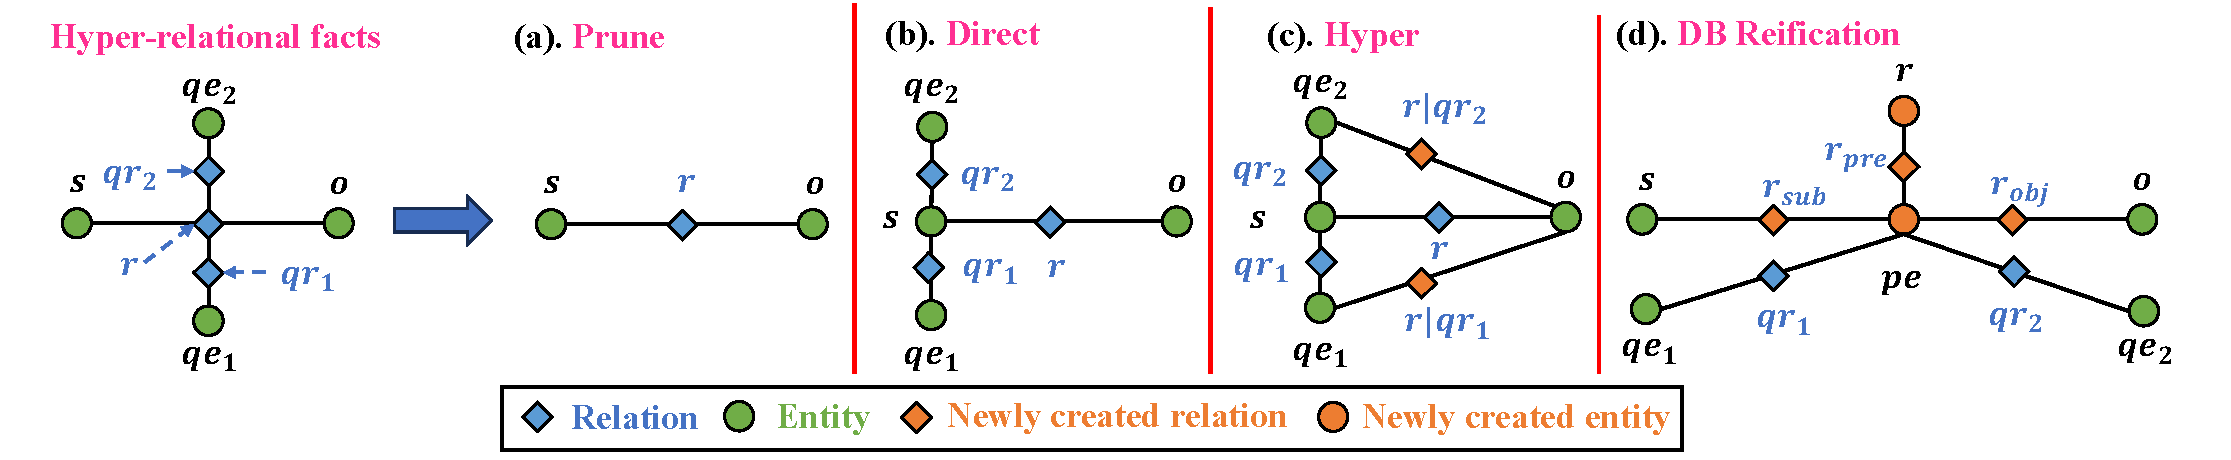
\includegraphics[width=\linewidth]{figures/hyperkg/decomp_new.pdf}
\caption{Original comparison of hyper-relational decomposition methods. Prune retains the main triple; Direct adds subject--qualifier links; Hyper adds combined relations; database reification introduces auxiliary objects. Reproduced from Fig.~1 of the CIKM study~\cite{bg-hyperkg}.}
\label{fig:background:decomposition}
\end{figure}

The association of a qualifier with a statement is especially relevant when a subject participates in several facts using the same relation. In the education example, a degree describes one university attendance statement. A collection of subject--degree and subject--university triples exposes the entities but changes the representation of which degree qualifies which attendance fact. A model following ordinary graph paths then receives the transformed connections. The Hyper method supplies additional connections intended to retain more of these associations, whereas a qualifier integrator receives the main fact and its qualifier pairs together. This comparison places information preservation at the interface between the data representation and the computation that follows it. It concerns the semantic organization of the input as well as its vocabulary.

The experiments compare conventional KGE models under these transformations with specialized HKGE models. Some GNN-based KGE configurations obtain scores comparable to specialized methods on Cleaned JF17k and WD50k. The observation motivates an examination of the represented information and the architecture receiving it. In particular, adding qualifier-derived edges can change the paths followed by a graph encoder. Preserving more items in a converted graph therefore changes the model's computational input as well as the nominal amount of stored information.

\subsection{Qualifier Capture and Graph Reception}

The analysis separates qualifier capture from graph reception. Qualifier capture concerns how the model represents qualifier pairs and their association with the main statement. Graph reception concerns how it receives information from the wider graph, including dependencies beyond one fact. Models operating on a fact in isolation have a different receptive field from graph encoders that propagate information across several hops. These properties are visible in the operations used to construct representations.

CompGCN jointly models entity and relation representations in a multi-relational graph~\cite{bg-compgcn}. NBFNet aggregates path information for link prediction~\cite{bg-nbfnet}. Their graph computations offer different ways to receive neighborhood and path information after decomposition. The CIKM analysis also identifies an information-compression issue when qualifier information is aggregated into fixed-size main-triple representations. Wider graph reception and qualifier integration consequently concern complementary parts of the architecture. The study evaluates designs that retain both sources for prediction.

FormerGNN combines a Transformer-based qualifier integrator operating on the original hyper-relational facts with a graph encoder operating on the pruned main-triple graph. The graph encoder generates a topology representation for the subject. The model concatenates this representation with representations of the main triple and qualifier pairs and passes them to a Transformer decoder. This organization supplies qualifier and graph information jointly to the prediction stage. In the reported configuration, HyperFormer provides the qualifier integrator and NBFNet provides the graph encoder~\cite{bg-hyperformer,bg-nbfnet}.

\subsection{Representative Published Evidence}

Table~\ref{tab:background:formergnn} reproduces the Cleaned JF17k and WD50k columns of the study's Table~6. It retains all seven model rows and all three metrics for those datasets. MRR measures mean reciprocal rank, and H@1 and H@10 measure whether the target entity appears within the corresponding rank cutoff. These are link-prediction measures, distinct from the annotation and answer metrics of the later chapters.

\begin{table}[tbp]
\centering
\caption{Projection of the CIKM study's Table~6 onto Cleaned JF17k and WD50k. All model rows and the original metric precision are retained; the original bold and underline markings indicate best and second-best values.}
\label{tab:background:formergnn}
\small
\begin{tabular}{lrrrrrr}
\toprule
&\multicolumn{3}{c}{Cleaned JF17k}&\multicolumn{3}{c}{WD50k}\\
\cmidrule(lr){2-4}\cmidrule(lr){5-7}
Model&MRR&H@1&H@10&MRR&H@1&H@10\\
\midrule
StarE&0.381&0.284&0.577&0.346&0.268&0.494\\
QUAD&0.402&0.305&0.602&0.349&0.275&0.487\\
HAHE&0.405&0.310&0.585&0.360&0.288&0.496\\
HyperFormer&\underline{0.425}&\underline{0.328}&0.613&\underline{0.372}&\underline{0.293}&0.522\\
NBFNet + Prune&0.415&0.313&\textbf{0.630}&0.360&0.271&\textbf{0.530}\\
CompGCN + Hyper&0.389&0.294&0.590&0.350&0.277&0.488\\
FormerGNN&\textbf{0.432}&\textbf{0.335}&\underline{0.624}&\textbf{0.377}&\textbf{0.299}&\underline{0.527}\\
\bottomrule
\end{tabular}
\end{table}

FormerGNN obtains MRR 0.432 on Cleaned JF17k and 0.377 on WD50k, compared with HyperFormer's 0.425 and 0.372. NBFNet + Prune has the highest H@10 in both selected datasets, at 0.630 and 0.530. The table therefore supports a metric-specific comparison. The experiment uses a single NVIDIA A100-40GB GPU. Parameters follow the original repositories or are selected by grid search when dataset-specific settings are unavailable. For comparisons involving CompGCN, the study replaces its decoder with a Transformer to align it with the corresponding HKGE configurations.

The complete published comparison also includes Wikipeople and FBAUTO, where dataset characteristics and metric rankings differ. The selected table illustrates graph reception and qualifier integration on these two datasets. The research establishes that the organization of graph information can matter beyond retaining the same entity and relation vocabulary. Its connection to this thesis is the design question of which relationships remain available to a model after evidence transformation. FormerGNN is a separate KG embedding framework; the four language-model systems use the structures and interfaces defined in their own chapters.

\section{Research Questions Emerging from the Background}
\label{sec:background:questions}

The preceding work identifies several places where structure can influence model inputs. Table understanding needs evidence that matches both the values and the task's type vocabulary. Dynamic classification needs an index that incorporates newly available label information and retrieves appropriate alternatives for the current text. Open-ended text generation needs a selection rule that can organize connected facts and retain their source context. Multimodal generation adds semantic matching across heterogeneous evidence and the cost of processing that evidence as model context.

The four research chapters address these conditions in sequence. Chapter~\ref{ch:kglink} studies external KG evidence and supervised type representations. Chapter~\ref{ch:gorag} studies connected candidate-label retrieval and online index updates. Chapter~\ref{ch:agrag} studies influence-aware connected evidence selection with hybrid passages. Chapter~\ref{ch:mgrag} studies query-aware multimodal graph construction, semantic path matching, and graph-aware KV recomputation. The hyper-relational study provides a related analysis of information preservation. The shared concern is how a representation exposes task-relevant evidence to the computation that uses it.
